\documentclass[preprint,3p,11pt,sort]{elsarticle}
\usepackage[utf8]{inputenc}

% Maths
\usepackage{amsmath,amssymb,amsfonts} % Equations
\usepackage{textcomp, gensymb} % Symbol: \degree

% Tables
\usepackage{multirow}

% Images
\usepackage{graphicx}
\usepackage{caption} % Improvements to figures, extends functionality with more options
\usepackage{placeins} % \FloatBarrier

% Text Modification
\usepackage[colorlinks=true, allcolors=blue]{hyperref} % Hyperlinks

% Figure & table ref
\newcommand{\figref}[1]{Fig.~\ref{#1}}
\newcommand{\tbref}[1]{Table~\ref{#1}}
\newcommand{\secref}[1]{Section~\ref{#1}}


%%%%%%%%%%%%%%%%%%%%%%%%%%%%%%%%%%%%%%%%%%%%%%%%%%%%%%%%%%%%%%%%%%%%%%%%%%%%%%%%%
%%%%%%%%%%%%%%%%%%%%%%%%%%%%%%%%%%%%%%%%%%%%%%%%%%%%%%%%%%%%%%%%%%%%%%%%%%%%%%%%%
\journal{JournalName}
\begin{document}
\begin{frontmatter}

\title{My Example Manuscript}

\nonumnote{Abbreviations: aaa}

\begin{abstract}
    This is an example manuscript. It showcases a few common latex features so that I can show how latexdiff interacts with them.
\end{abstract}

\begin{keyword}
    a \sep b \sep c \sep d
\end{keyword}

\end{frontmatter}

%%%%%%%%%%%%%%%%%%%%%%%%%%%%%%%%%%%%%%%%%%%%%%%%%%%%%%%%%%%%%%%%%%%%%%%%%%%%%%%%%
%%%%%%%%%%%%%%%%%%%%%%%%%%%%%%%%%%%%%%%%%%%%%%%%%%%%%%%%%%%%%%%%%%%%%%%%%%%%%%%%%
\section{Introduction} \label{sec:intro}
This is an example manuscript.

The structure of this article is as follows: \secref{sec:mySection} showcases the use of SSSSR sections. \secref{sec:ContentTypes} shows how to display many different types of content.


%%%%%%%%%%%%%%%%%%%%%%%%%%%%%%%%%%%%%%%%%%%%%%%%%%%%%%%%%%%%%%%%%%%%%%%%%%%%%%%%%
%%%%%%%%%%%%%%%%%%%%%%%%%%%%%%%%%%%%%%%%%%%%%%%%%%%%%%%%%%%%%%%%%%%%%%%%%%%%%%%%%
\section{Displaying Sections} \label{sec:mySection}
This section has many subsections, which I can refer to by their labels. e.g. \secref{sec:mySection}, \secref{ssec:mySubsectionA}, and \secref{ssec:mySubsectionB}. Labeling sections is optional. Labels may be anything, but must be unique (hence my naming convention).

%%%%%%%%%%%%%%%%%%%%%%%%%%%%%%%%%%%%%%%%%%%%%%%%%%%%%%%%%%%%%%%%%%%%%%%%%%%%%%%%%
\subsection{My Subsection A} \label{ssec:mySubsectionA}
Example text.


%%%%%%%%%%%%%%%%%%%%%%%%%%%%%%%%%%%%%%%%%%%%%%%%%%%%%%%%%%%%%%%%%%%%%%%%%%%%%%%%%
\subsection{My Subsection B} \label{ssec:mySubsectionB}
Example text.


%%%%%%%%%%%%%%%%%%%%%%%%%%%%%%%%%%%%%%%%%%%%%%%%%%%%%%%%%%%%%%%%%%%%%%%%%%%%%%%%%
%%%%%%%%%%%%%%%%%%%%%%%%%%%%%%%%%%%%%%%%%%%%%%%%%%%%%%%%%%%%%%%%%%%%%%%%%%%%%%%%%
\section{Displaying Different Types of Content} \label{sec:ContentTypes}


%%%%%%%%%%%%%%%%%%%%%%%%%%%%%%%%%%%%%%%%%%%%%%%%%%%%%%%%%%%%%%%%%%%%%%%%%%%%%%%%%
\subsection{Citations}
This is a citation \cite{example1}, and this is another \cite{example1,example2,example4,example5}.


%%%%%%%%%%%%%%%%%%%%%%%%%%%%%%%%%%%%%%%%%%%%%%%%%%%%%%%%%%%%%%%%%%%%%%%%%%%%%%%%%
\subsection{Lists}
An example list is as follows:

\begin{enumerate}
    \item This is a list
    \item This is a list
    \item This is a list
\end{enumerate}


%%%%%%%%%%%%%%%%%%%%%%%%%%%%%%%%%%%%%%%%%%%%%%%%%%%%%%%%%%%%%%%%%%%%%%%%%%%%%%%%%
\subsection{Figures}
This is a figure reference: \figref{fig:Example1}, and this is another \figref{fig:Example2}.

If you have mathematical symbols in your figures and you're using inkscape, you can input latex maths into the figure with: Extensions > Render > Formula (pdflatex).

\begin{figure}
	\centering
	\centerline{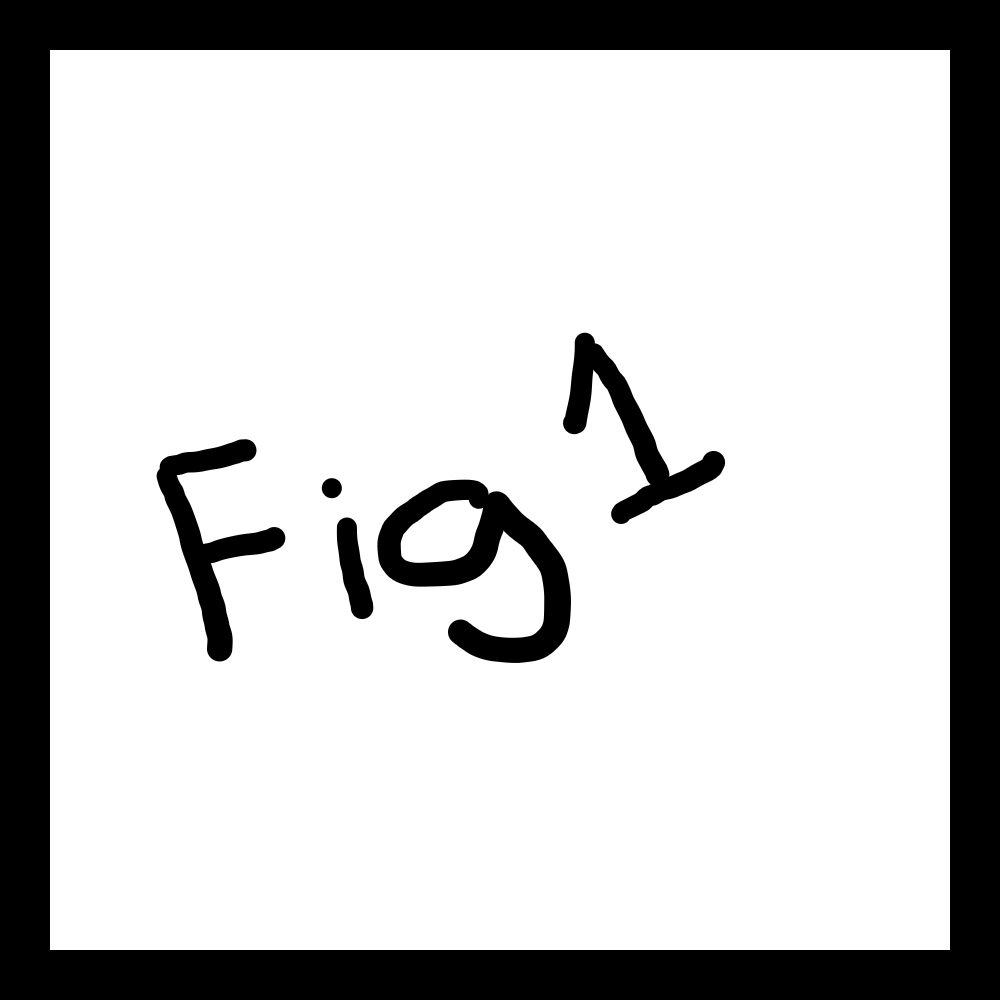
\includegraphics[width=\textwidth,keepaspectratio]{Figures/ExampleFigure1.png}}
	\caption{Embed your graphics as pdf. Lovely vector graphics! If I see any jpeg text I am sad.}
	\label{fig:Example1}
\end{figure}

\begin{figure}
	\centering
	\centerline{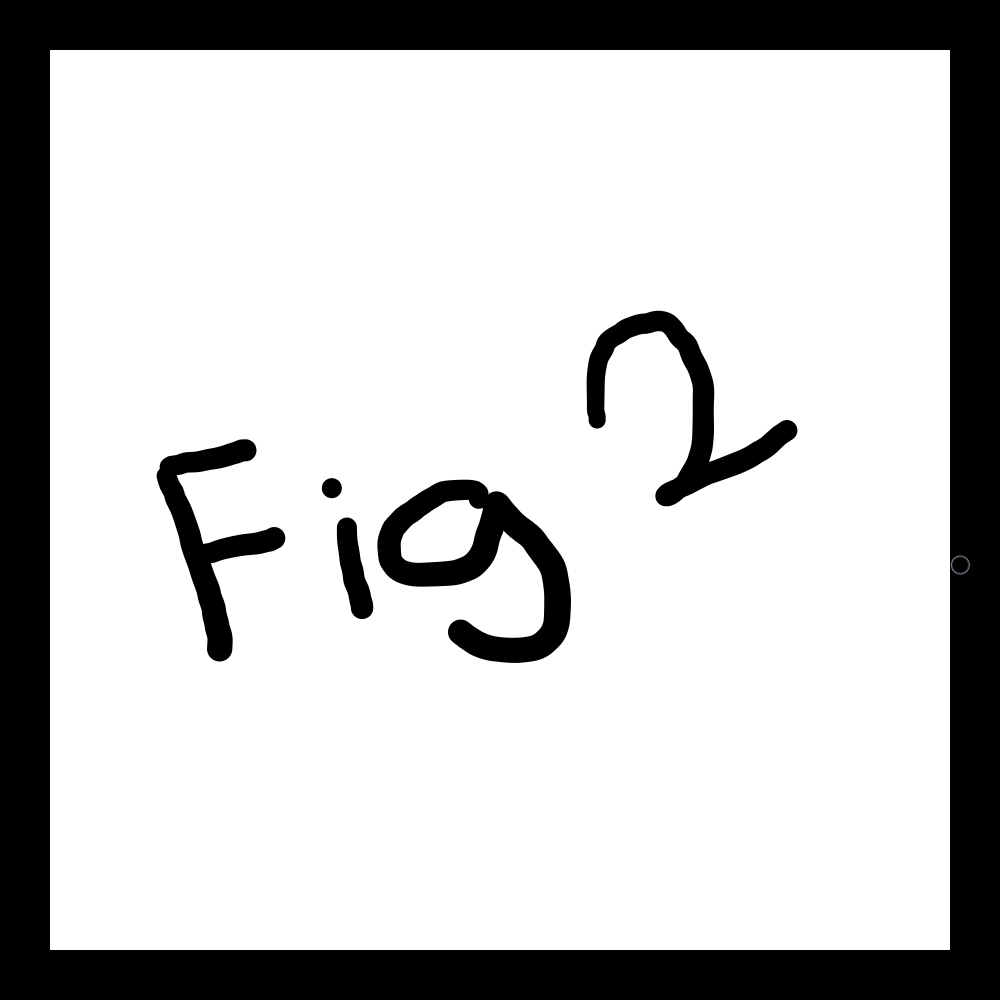
\includegraphics[width=\textwidth,keepaspectratio]{Figures/ExampleFigure2.png}}
	\caption{This is a caption.}
	\label{fig:Example2}
\end{figure}


%%%%%%%%%%%%%%%%%%%%%%%%%%%%%%%%%%%%%%%%%%%%%%%%%%%%%%%%%%%%%%%%%%%%%%%%%%%%%%%%%
\subsection{Equations}
This is an equation reference: \eqref{eq:myEq}.

\begin{equation} \label{eq:myEq}
    a = 3
\end{equation}

where $a$ is a variable.


%%%%%%%%%%%%%%%%%%%%%%%%%%%%%%%%%%%%%%%%%%%%%%%%%%%%%%%%%%%%%%%%%%%%%%%%%%%%%%%%%
\subsection{Tables}
This is a table reference: \tbref{tb:myTable}.

This is a fairly basic table. See threeparttable if you want table notes (footnotes for tables).

\begin{table}[!h]
    \centering
    \begin{tabular}{llll}
        \hline
        & & \multicolumn{2}{l}{Measurement error}\\
        Measurement & Unit & Mean & Standard deviation\\
        \hline
        $x_n$ & mm & 5.2 & 8.6\\
        $y_n$ & mm & 3.5 & 3.0\\
        $z_n$ & mm & -6.5 & 9.1\\
        $\theta_q$ & degrees & 1.6$\degree$ & 2.9$\degree$\\
        \hline
        \end{tabular}
    \caption{Average measurement error over all 99 successful measurements. $(x_n, y_n, z_n)$ are defined somewhere else. $\theta_q$ is the rotational misalignment as a quaternion angular distance.}
    \label{tb:myTable}
\end{table}


%%%%%%%%%%%%%%%%%%%%%%%%%%%%%%%%%%%%%%%%%%%%%%%%%%%%%%%%%%%%%%%%%%%%%%%%%%%%%%%%%
%%%%%%%%%%%%%%%%%%%%%%%%%%%%%%%%%%%%%%%%%%%%%%%%%%%%%%%%%%%%%%%%%%%%%%%%%%%%%%%%%
\section{Conclusions and Future Work} \label{sec:conclusions}
Thus ends the example manuscript.

I can't be bothered to recommend future work.


\FloatBarrier
%%%%%%%%%%%%%%%%%%%%%%%%%%%%%%%%%%%%%%%%%%%%%%%%%%%%%%%%%%%%%%%%%%%%%%%%%%%%%%%%%
%%%%%%%%%%%%%%%%%%%%%%%%%%%%%%%%%%%%%%%%%%%%%%%%%%%%%%%%%%%%%%%%%%%%%%%%%%%%%%%%%
\bibliographystyle{elsarticle-num}
\bibliography{Bibliography/Bibliography.bib}

%%%%%%%%%%%%%%%%%%%%%%%%%%%%%%%%%%%%%%%%%%%%%%%%%%%%%%%%%%%%%%%%%%%%%%%%%%%%%%%%%
%%%%%%%%%%%%%%%%%%%%%%%%%%%%%%%%%%%%%%%%%%%%%%%%%%%%%%%%%%%%%%%%%%%%%%%%%%%%%%%%%
\end{document}
\endinput

